% Description du contenu du rapport à rendre pour l'UF temps réel en 4AE et 4IR
% Auteur : P.-E. Hladik 
% Institut : INSA de Toulouse
% Tuteur : kevin.delmas@onera.fr

\documentclass[11pt, a4paper]{paper}
\usepackage{a4wide,color}

\usepackage[utf8]{inputenc}
\usepackage[T1]{fontenc}
\usepackage[francais]{babel}
\usepackage{float}
\usepackage{graphicx}
\usepackage{amssymb}
\usepackage{hyperref}

\usepackage{amstext}
\usepackage{amsmath}

\usepackage[dvipsnames]{xcolor}

\usepackage{placeins}

\newcounter{cptreq}

\usepackage{framed}

%% Sauts de page à chaque section
\usepackage{titlesec}
\newcommand{\sectionbreak}{\clearpage}

\title{{\Huge Rapport de projet De Stijl 2.0}\\
{\large version \today}\\
---\\
}
\author{
    {Théo BUENO (implémentation et tests, diagramme fonctionnel)}\\
    {Tangi DELANOË (conception et diagrammes d'activité, toutes fonctions)}\\
    {Adrian MEGA (conception et diagrammes d'activité, toutes fonctions)}\\
    {Jean THONGPHAN (conception et diagrammes d'activité, toutes fonctions)}\\
    {Tous (rédaction du compte-rendu)}
}

\begin{document}

%%%%%%%%%%%%%%
% PAGE DE GARDE
\maketitle

\tableofcontents

%%%%%%%%%%%%%%
% DEBUT DU RAPPORT
\newpage

%%%%%%%%%%%%%%%%%%%
% TRANSFORMATION AADL2XENO
\section{Transformation AADL vers Xenomai}
Dans cette section sont décrits les mécanismes que nous avons utilisés pour implémenter nos processus à partir de leur description en diagramme fonctionnel AADL, à l'aide des outils de Xenomai.

 % PORT D'EVENEMENT: LECTURE SEULE
\subsection{Port d’événement}

% INSTANCIATION PORT D'EVENEMENT: LECTURE SEULE
\subsubsection{Instanciation}
\label{event_sema}
Chaque port d'évènement a été instancié par un sémaphore.
Les sémaphores sont déclarés en variable globales, exportés avec un {\tt export} pour êtres accessibles par les tâches, et initialisés avec {\tt rt\_sem\_create}.

La création des sémaphores est réalisée au démarrage lors de l'appel de la fonction {\tt initStruct} depuis le {\tt main}.

Par exemple, pour l'événement {\tt startCamera}, sa déclaration est faite ligne 29 dans le fichier {\tt main.c} avec
\begin{verbatim}
  RT_SEM sem_startCamera;
\end{verbatim}
et son instanciation ligne 171 par 
\begin{verbatim}
if (err = rt_sem_create(&sem_startCamera, NULL, 0, S_FIFO)) {
    printf("Error semaphore create: %s\n", strerror(-err));
    exit(EXIT_FAILURE);
}
\end{verbatim}

% ENVOI PORT D'EVENEMENT: LECTURE SEULE
\subsubsection{Envoi d’un événement}
Pour signaler un évènement, on utilise la primitive {\tt rt\_sem\_v} qui permet d'augmenter le nombre de ressources disponibles du sémaphore de 1. On notifie donc d'un nouvel évènement par un jeton qui peut être traité par une tâche.

Par exemple, pour l'évènement {\tt startCamera}, on notifie la tâche de démarrage de la caméra qu'elle doit démarrer son traitement dans le fichier {\tt functions.cpp} à la ligne 250:
\begin{verbatim}
  rt_sem_v(&sem_startCamera);
\end{verbatim}

Lorsqu'un évènement doit être notifié à plusieurs tâches, on utilise toujours une sémaphore mais avec la primitive {\tt rt\_sem\_broadcast}. Cette fonction débloque toutes les tâches qui étaient déjà en attente d'une notification de cet évènement.

Par exemple, dans le fichier {\tt main.c} à la ligne 112 avec le sémaphore {\tt sem\_barrier} qui permet de synchroniser le démarrage de toutes les tâches:
\begin{verbatim}
    rt\_sem_broadcast(&sem\_barrier);
\end{verbatim}

% RECEPTION PORT D'EVENEMENT: LECTURE SEULE
\subsubsection{Réception d’un événement}
Pour attendre un évènement, on utilise la primitive {\tt rt\_sem\_p} qui essaye de prendre un jeton du sémaphore. On attend donc activement un évènement tant qu'un jeton n'est pas disponible dans le sémaphore.

Par exemple, pour l'évènement {\tt startCamera}, la tâche de démarrage de la caméra attend de démarrer son traitement dans le fichier {\tt functions.cpp} à la ligne 357:
\begin{verbatim}
  rt_sem_p(&sem_startCamera, TM_INFINITE);
\end{verbatim}

Le flag {\tt TM\_INFINITE} indique que l'attente se fait sans timeout, et bloque ainsi la tâche tant que l'évènement n'est pas levé.

On utilise également un timeout lorsqu'on ne souhaite pas que l'attente soit infinie, par exemple lorsque la tâche a d'autres traitements à effectuer. C'est le cas pour la tâche de traitement des images {\tt th\_pictures} qui vérifie périodiquement si elle doit rechercher une nouvelle arène avec l'évènement {\tt sem\_probeArena}.

Ainsi, à la ligne 95 de {\tt functions.cpp} on a:
\begin{verbatim}
    /* 1ms pour attendre probeArena */
    if(rt_sem_p(&sem_probeArena, 1000000) == 0)
    {
\end{verbatim}

Ce code vérifie l'évènement probeArena pendant 1ms avant de continuer son traitement. Si l'évènement a été levé, alors la function retourne 0 (pas d'erreur) et la recherche de l'arène commence. Sinon, une erreur de timeout a été levée et donc la tâche continue son traitement sans changer l'arène.

% DONNEE PARTAGEE: LECTURE_SEULE
\subsection{Donnée partagée}
Les données partagées sont des variables globales protégées par des mutex.

% INSTANCIATION DONNEE PARTAGEE: LECTURE_SEULE
\subsubsection{Instanciation}

On déclare les variables globales (les données partagées) et les mutex les protégeant avec des déclarations de variables globales.

À la ligne 45 de {\tt main.cpp}:
\begin{verbatim}
RT_MUTEX mutex_robotStarted;
\end{verbatim}

puis à la ligne 70:
\begin{verbatim}
int robotStarted = 0;
\end{verbatim}

Les mutex doivent aussi êtres initialisés à l'aide de {\tt rt\_mutex\_create}. initStruct() permet la création des mutex, par exemple à la ligne 125 de {\tt main.cpp}:

\begin{verbatim}
if (err = rt_mutex_create(&mutex_robotStarted, NULL)) {
    printf("Error mutex create: %s\n", strerror(-err));
    exit(EXIT_FAILURE);
}
\end{verbatim}

% LECTURE/ECRITURE DONNEE PARTAGEE: LECTURE SEULE
\subsubsection{Accès en lecture et écriture}
L'accès à une section critique est protégé par un mutex. Les ressources ou certains états sont eux protégés par des sémaphores, qui peuvent servir comme ports d'évènements ou de synchronisation.

Pour accéder à une donnée partagée, il faut au préalable verrouiller son mutex. Un mutex ne peut être verouillé qu'une seule fois, sinon la primitive de verrouillage {\tt rt\_mutex\_acquire} place l'appelant en attente jusqu'à libération du mutex.

Par exemple, pour modifier le statut du robot la tâche de démarrage du robot à la ligne 409 de {\tt functions.cpp} fait:

\begin{verbatim}
rt_mutex_acquire(&mutex_robotStarted, TM_INFINITE);
robotStarted = 1;
rt_mutex_release(&mutex_robotStarted);
\end{verbatim}

La variable robotStarted n'est modifiée que lorsque le verrouillage de son mutex est garanti. Puis le mutex est libéré avec {\tt mutex\_robotStarted}.

% PORT D'EVENEMENT-DONNEES: LECTURE SEULE
\subsection{Ports d’événement-données}
Pour l'implémentation des canaux d'évènement-données, nous avons utilisés différents outils de Xenomai. La tâche {\tt sendToMon} utilise une file de message qui permet de transmettre une donnée de manière asynchrone et transparente.

Nos autres tâches utilisent des mécanismes différents quand il n'y a pas de possibilité d'évènements-données multiples à traiter. C'est le cas par exemple du thread {\tt th\_pictures} de traitement des images, qui reçoit une confirmation ou une infirmation sur l'arène sélectionnée à l'aide d'une variable partagée dont la consultation est déclenchée par un sémaphore, à la ligne 105 de {\tt functions.cpp}:

\begin{verbatim}
// On attend une confirmation/infirmation du moniteur
rt_sem_p(&sem_probeArena, TM_INFINITE);
rt_mutex_acquire(&mutex_arene, TM_INFINITE);
if(confirmationArene == 1)
{
    // L'arène est confirmée
    areneConfirmee = 1;
\end{verbatim}

La suite ne décrit pas ce cas puisqu'il est déjà couvert par les autres sections concernant les ports évènements et les variables partagées.

% INSTANCIATION PORT D'EVENEMENT-DONNEES: LECTURE SEULE
\subsubsection{Instanciation}
Pour instancier une file de message on la déclare en variable globale, avant de l'initialiser avec la primitive {\tt rt\_queue\_create}.

Par exemple ligne 64 de {\tt main.cpp}:
\begin{verbatim}
    RT_QUEUE q_messageToMon;
\end{verbatim}

puis ligne 230 de {\tt main.cpp}:
\begin{verbatim}
/* Creation des files de messages */
if (err = rt_queue_create(&q_messageToMon, "toto",
                        MSG_QUEUE_SIZE * sizeof (MessageToRobot),
                        MSG_QUEUE_SIZE, Q_FIFO)) {
    printf("Error msg queue create: %s\n", strerror(-err));
    exit(EXIT_FAILURE);
}
\end{verbatim}

% ENVOI PORT D'EVENEMENT-DONNEES: LECTURE SEULE
\subsubsection{Envoi d’une donnée}
L'écriture des données à la fin d'une queue à se fait à l'aide de la fonction {\tt write\_in\_queue}.

Par exemple ligne 122 de {\tt functions.cpp} avec l'envoi d'un non-acquittement au moniteur:
\begin{verbatim}
// On a pas trouvé d'arène
MessageToMon msg;
set_msgToMon_header(&msg, HEADER_STM_NO_ACK);
write_in_queue(&q_messageToMon, msg);
\end{verbatim}

% RECEPTION PORT D'EVENEMENT-DONNEES: LECTURE SEULE
\subsubsection{Réception d’une donnée}
La réception des données écrites sur une queue est effectuée avec {\tt rt\_queue\_read}.

Par exemple ligne 179 de {\tt functions.cpp} avec la lecture d'une donnée en attente de traitement dans la file d'envoi de messages vers le moniteur:
\begin{verbatim}
#ifdef _WITH_TRACE_
printf("%s : waiting for a message in queue\n", info.name);
#endif
if (rt_queue_read(&q_messageToMon, &msg, sizeof (MessageToRobot), TM_INFINITE) >= 0) {
#ifdef _WITH_TRACE_
    printf("%s : message {%s,%s} in queue\n", info.name, msg.header, msg.data);
#endif
\end{verbatim}

% THREAD: LECTURE SEULE
\subsection{Thread}
Les différentes tâches sont traitées par des threads du processus principal du superviseur.

% INSTANCIATION THREAD: LECTURE SEULE
\subsubsection{Instanciation et démarrage}

La création de chaque tâche est effectuée dès le démarrage de l'application par initStruct().
Par exemple pour la création du thread de démarrage du robot à la ligne 205 de {\tt main.cpp}:
\begin{verbatim}
if (err = rt_task_create(&th_startRobot, "th_startRobot", 0, PRIORITY_TSTARTROBOT, 0)) {
    printf("Error task create: %s\n", strerror(-err));
    exit(EXIT_FAILURE);
}
\end{verbatim}
Cette fonction initialise le thread, lui donne un nom qui permet de l'identifier lors des fonctions d'affichage à la console et lui affecte une priorité.

La fonction startTasks() démarre les threads qui ont été initialisés par initStruct(). Par exemple à la ligne 251 de {\tt main.cpp}:
\begin{verbatim}
if (err = rt_task_start(&th_startRobot, &f_startRobot, NULL)) {
        printf("Error task start: \%s", strerror(-err));
        exit(EXIT\_FAILURE);
}
\end{verbatim}
 
% CODE THREAD: LECTURE SEULE
\subsubsection{Code à exécuter}
Au démarrage de la tâche, une fonction comme point d'entrée du thread est spécifiée dans l'appel à {\tt rt\_task\_start}. Pour tous les threads il s'agit de la fonction de traitement correspondance à la tâche, dans {\tt functions.cpp}. Toutes ces fonctions implémentent en principe une boucle infinie: c'est la boucle de traitement de la tâche.

Pour le thread de démarrage du robot il s'agit de la fonction {\tt f\_startRobot}, que l'on trouve déclarée à partir de la ligne 383 de {\tt functions.cpp}:

\begin{verbatim}
void f_startRobot(void * arg) {
    int err;

    /* INIT */
    RT_TASK_INFO info;
    rt_task_inquire(NULL, &info);
    printf("Init %s\n", info.name);
    rt_sem_p(&sem_barrier, TM_INFINITE);

    while (1) { /* boucle de traitement */
#ifdef _WITH_TRACE_
        printf("%s : Wait sem_startRobot\n", info.name);
#endif
        rt_sem_p(&sem_startRobot, TM_INFINITE);
        ...
\end{verbatim}

% PRIORITE THREAD: LECTURE SEULE
\subsubsection{Niveau de priorités}
Les thread ayant un indice de priorité le plus élevé seront celles qui seront executées en priorité par l'ordonnanceur du système Xenomai.

Notre stratégie de configuration des priorités est de placer en premier les tâches permettant l'initialisation des sous-systèmes ainsi que la communication. On retrouvera notamment les threads lié au groupe de gestion du moniteur et de démarrage du robot et de la caméra. Ces threads sont prioritaires car le bon fonctionnement des autres tâches en dépendent.

Ensuite, les threads lié à la gestion du robot et de la caméra ont une priorité intermédiaire, car moins importants.

Enfin l'affichage de la batterie et l'envoi périodique d'image auront tout deux une priorité faible, car l'état de la batterie n'est pas une fonctionnalité importante. Le traitement des images quant à lui est une opération assez lourde, il ne faut donc pas qu'il occupe l'unité centrale trop longtemps au détriment des autres threads, ce qui pourrait créer une situation de famine.

% PERIODICITE THREAD: LECTURE SEULE
\subsubsection{Activation périodique}
Certaines fonctionnalités nécessitent une certaine périodicité, tel que l'envoi d'image par exemple. Pour ces tâches il est donc nécessaire de mettre en place un timer pour garantir leur exécution périodique. Ce timer est en quelque sorte un sémaphore automatique, qui se débloque avec une période donnée.

La mise en place de ce timer est faite par la fonction {\tt rt\_task\_set\_periodic}.
Par exemple, pour la tâche d'envoi du statut de la batterie à la ligne 484 de {\tt functions.cpp}:

\begin{verbatim}
/* Période de 500 ms */
rt_task_set_periodic(NULL, TM_NOW, 500000000);
while (1) { ... }
\end{verbatim}

% THREAD EVENEMENTIEL: LECTURE SEULE
\subsubsection{Activation événementielle}
Plusieurs moyens sont mis en {\oe}uvre dans l'implémentation sous Xenomai pour gérer les activations événementielles d'un thread AADL. 

\begin{description}
\item[Sémaphores] Les sémaphores sont utilisés pour notifier un évènement à une tâche, tel que décrit à la section \ref{event_sema}. C'est le cas notamment du reset du superviseur, déclenché lors de la perte de la communication avec celui-ci.

À la ligne 225 de {\tt functions.cpp} la notification:
\begin{verbatim}
// Receive error
if(err <= 0)
{
#ifdef _WITH_TRACE_
    printf("%s : error receiving message from monitor\n", info.name);
#endif
    /* signalement d'une erreur critique nécessisant redémarrage du superviseur */
    rt_sem_v(&sem_serverKo); /* notification */
    pause();
}
\end{verbatim}

Et à la ligne de 14 {\tt functions.cpp} le traitement évènementiel:
\begin{verbatim}
#ifdef _WITH_TRACE_
    printf("%s: ready to reset supervisor\n", info.name);
#endif
    
rt_sem_p(&sem_serverKo, TM_INFINITE); /* attente évènement */

printf("%s: /!\\ monitor is unreachable, resetting supervisor /!\\\n", info.name);
\end{verbatim}

\item[Variables partagées] L'état de certaines variables partagées déclenchent l'activation de traitements spécifiques. C'est le cas par exemple de comFails qui est un compteur de trames perdues lors de la communication avec le robot, à la ligne 412 de {\tt functions.cpp}:

\begin{verbatim}
while(1){
    rt_mutex_acquire(&mutex_comFails, TM_INFINITE);
    if(comFails > 3) /* Branchement sur valeur de variable partagée */
    {
        rt_mutex_release(&mutex_comFails);
        ...
        /* On indique aux autres threads que le robot est arreté */
        /* On sort de la boucle secondaire pour se remettre en attente */
        /* d'une demande de connexion */
    }                
    rt_mutex_release(&mutex_comFails);
}
\end{verbatim}

\item[Files de messages] Le threads de communication avec le moniteur {\tt sendToMon} utilise une file de message pour déclencher un traitement évènementiel avec des données.

À la ligne 179 de {\tt functions.cpp}:
\begin{verbatim}
#ifdef _WITH_TRACE_
printf("%s : waiting for a message in queue\n", info.name);
#endif
if (rt_queue_read(&q_messageToMon, &msg, sizeof (MessageToRobot),
                                                    TM_INFINITE) >= 0) {
#ifdef _WITH_TRACE_
    printf("%s : message {%s,%s} in queue\n", info.name, msg.header, msg.data);
#endif
\end{verbatim}
\end{description}

% CONCEPTION
\section{Conception}

% VUE GENERAL DU SYSTEME
\subsection{Diagramme fonctionnel général}

\begin{figure}[H]
\label{fig:diag_fonc_gen}
\begin{center} 
% format paysage, au maximum de taille
{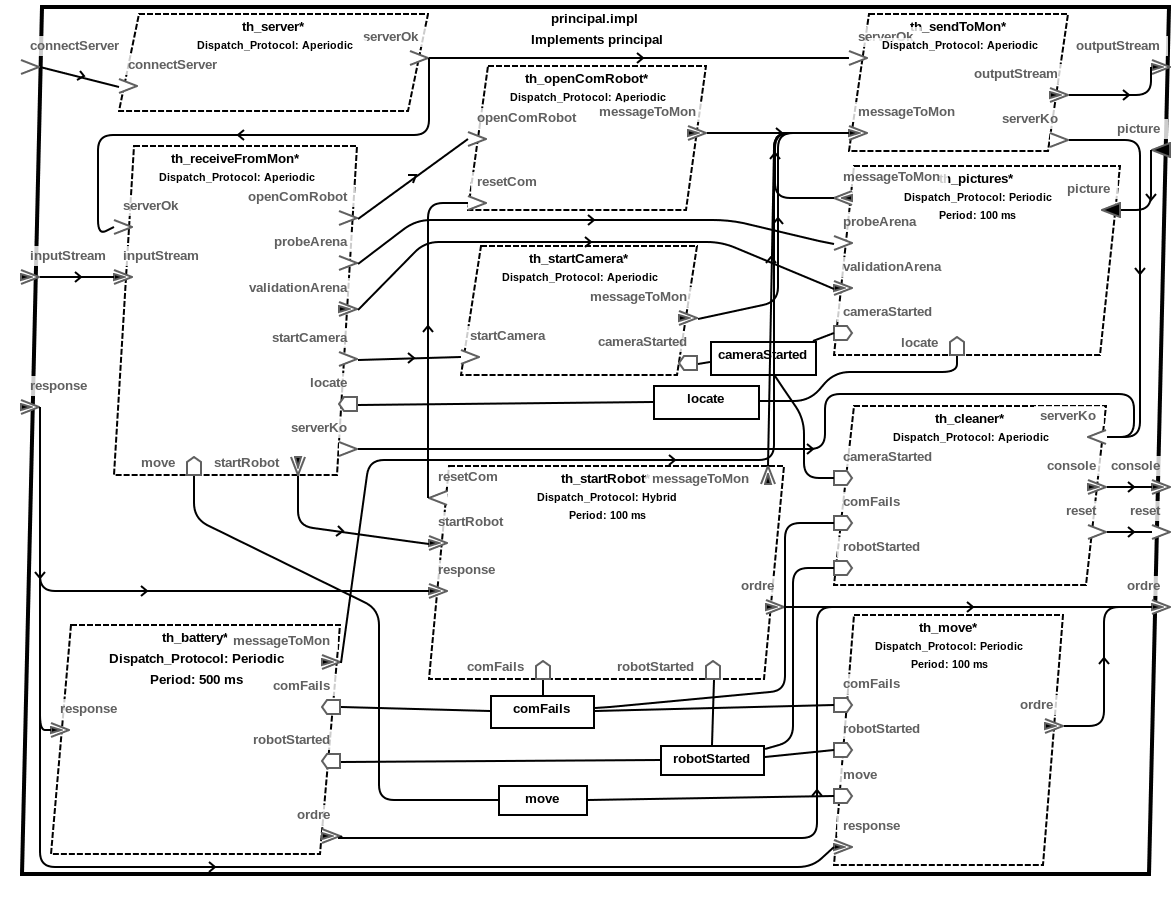
\includegraphics[height=0.65\textheight,angle=90]{./figures-pdf/diagramme_aadl_final.png}} 
{\caption{Diagramme fonctionnel du système}}
\end{center}
\end{figure}

\begin{figure}[H]
\label{fig:diag_fonc_gen_blocks}
\begin{center} 
% format paysage, au maximum de taille
{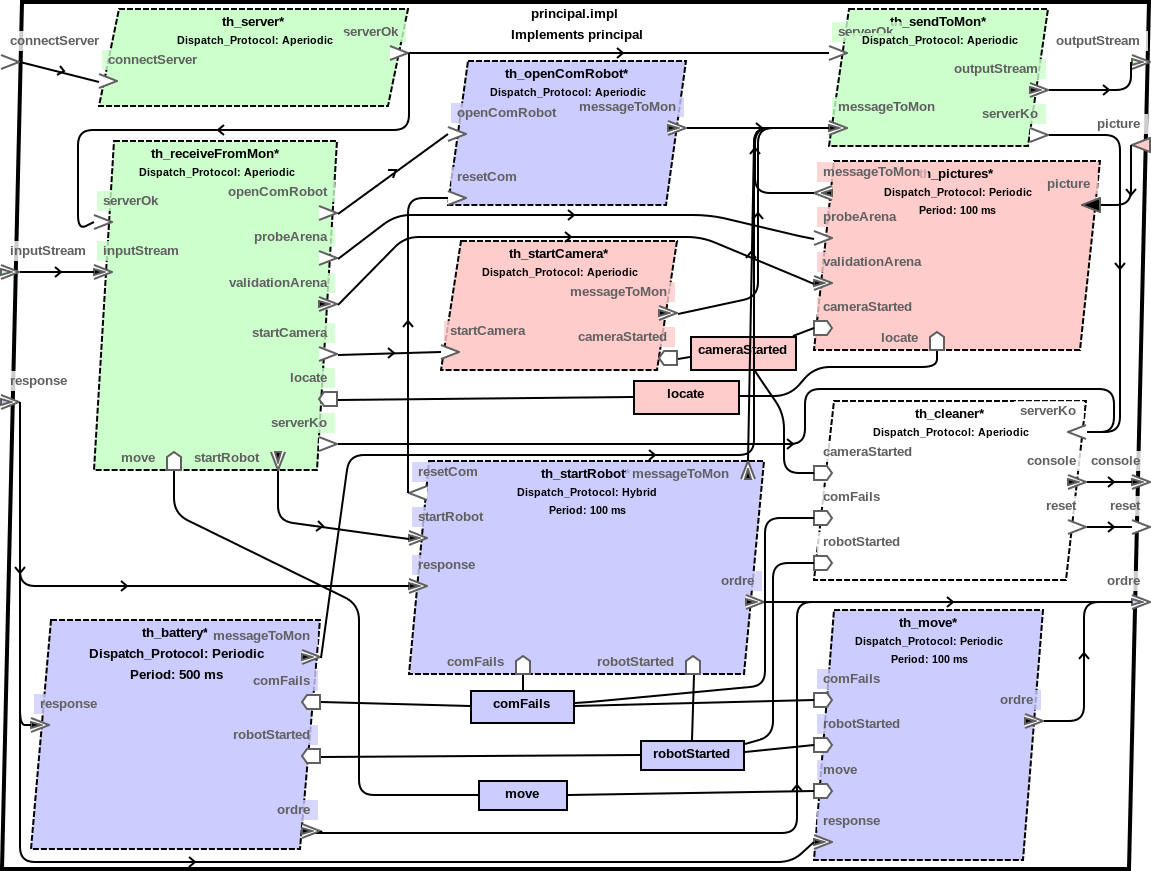
\includegraphics[height=0.65\textheight,angle=90]{./figures-pdf/diagramme_aadl_final_colorise.png}} 
{\caption{Diagramme fonctionnel du système avec groupes de fonctionnalités coloriés}}
\end{center}
\end{figure}

% DIAGRAMME FONCTIONNEL GT MONITEUR
\subsection{Groupe de threads gestion du moniteur}

% DIAGRAMME FONCTIONNEL GT MONITEUR: TODO
\subsubsection{Diagramme fonctionnel du groupe gestion du moniteur}
Voir \ref{fig:diag_fonc_gen_blocks}, {\color{green} blocs de couleur verte}.

% DESCRIPTION THREADS GT MONITEUR: LECTURE SEULE
\subsubsection{Description des threads du groupe gestion du moniteur}

\begin{table}[htp]
\begin{center}
\begin{tabular}{|p{4cm}|p{8.5cm}|p{2cm}|}
\hline
\bf Nom du thread &	\bf Rôle &	\bf Priorité \\
\hline
\hline

th\_server & Démarre les différents serveurs du superviseur &	30\\
\hline

th\_receiveFromMon & Reçoit et traite les messages provenant du moniteur  &	22\\
\hline

th\_sendFromMon & Envoi les messages des tâches vers le moniteur &	25\\
\hline

th\_cleaner &   Réinitialisation du superviseur &	30\\
\hline

\end{tabular}
\end{center}
\caption{Description des threads du groupe {\tt th\_group\_gestion\_moniteur}}
\label{tab:gt_moniteur}
\end{table}%

Les thread responsable de la bonne activité du groupe de gestion du moniteur sont les threads suivants:
\begin{description}
\item[th\_server] S'assure du bon démarrage du serveur NodeJS. Une fois le démarrage réussi, il fera ensuite appel à {\tt open\_server()} pour ouvrir le port de communication du superviseur. On notifie le succès de ces opérations avec l'évènement {\tt serverOk}
\item[th\_receiveFromMon] Permet la réception des messages en provenance du moniteur et répartie les informations vers les autres tâches
\item[th\_sendToMon] Permet l'envoi des messages en direction du moniteur par les tâches du processus
\item[th\_cleaner] Réinitialisation du superviseur en cas de perte de communication avec le moniteur
\end{description}

% DIAGRAMMES D'ACTIVITE GT MONITEUR
\subsubsection{Diagrammes d'activité  du groupe gestion du moniteur}

\begin{figure}[H]
\label{fig:th_server}
\begin{center}
{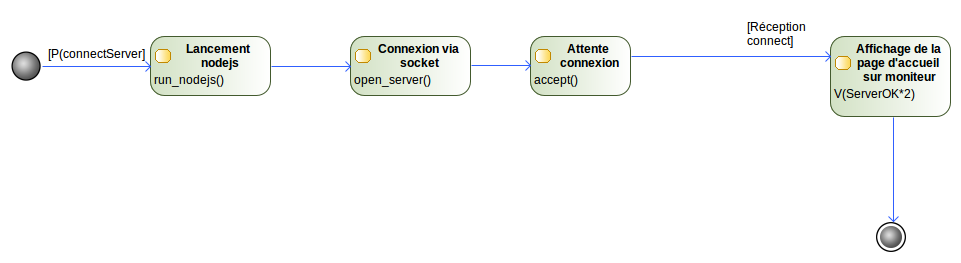
\includegraphics[width=1.0\textwidth]{./figures-pdf/th_server}}
{\caption{Diagramme d'activité du thread {\tt th\_server}}}
\end{center}
\end{figure}

\begin{figure}[H]
\label{fig:th_receiveFromMon}
\begin{center}
{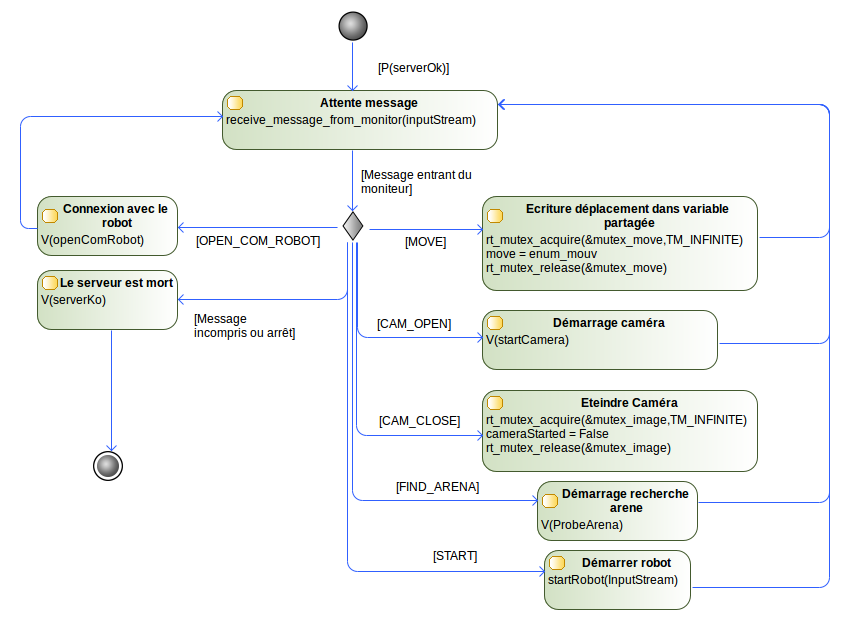
\includegraphics[width=0.8\textwidth]{./figures-pdf/th_receiveFromMon.png}}
{\caption{Diagramme d'activité du thread {\tt th\_receiveFromMon}}}
\end{center}
\end{figure}

\begin{figure}[H]
\label{fig:th_sendToMon}
\begin{center}
{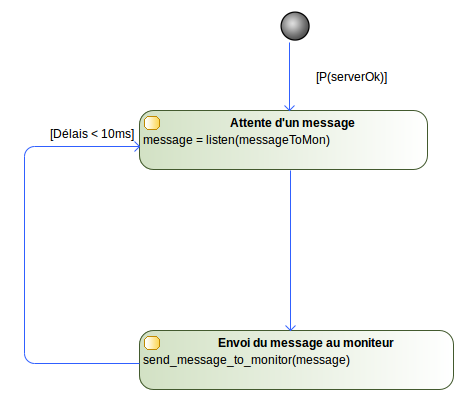
\includegraphics[width=0.7\textwidth]{./figures-pdf/th_sendToMon.png}}
{\caption{Diagramme d'activité du thread {\tt th\_sendToMon}}}
\end{center}
\end{figure}

\begin{figure}[H]
\label{fig:th_cleaner}
\begin{center}
{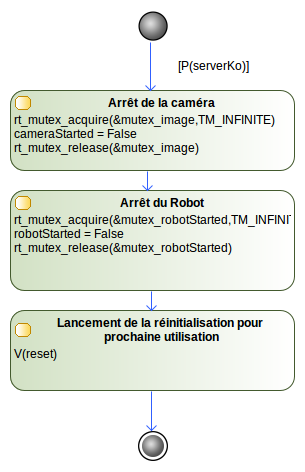
\includegraphics[width=0.5\textwidth]{./figures-pdf/th_cleaner}}
{\caption{Diagramme d'activité du thread {\tt th\_cleaner}}}
\end{center}
\end{figure}

% DIAGRAMME FONCTIONNEL GT VISION
\subsection{Groupe de threads vision}

% DIAGRAMME FONCTIONNEL GT VISION
\subsubsection{Diagramme fonctionnel du groupe vision}
Voir \ref{fig:diag_fonc_gen_blocks}, {\color{red} blocs de couleur rouge}.

% DESCRIPTION THREADS GT VISION: LECTURE SEULE
\subsubsection{Description des threads du groupe vision}

\begin{table}[H]
\begin{center}
\begin{tabular}{|p{3cm}|p{8.5cm}|p{2cm}|}
\hline
\bf Nom du thread &	\bf Rôle &	\bf Priorité \\
\hline
\hline
th\_startCamera & Démarre la caméra & 20\\
\hline
th\_pictures & Récupère, traite et envoi les images de la caméra toutes les 100 ms & 15\\
\hline

\end{tabular}
\end{center}
\caption{Description des threads du groupe {\tt th\_group\_vision}}
\label{tab:gt_vision}
\end{table}

Le thread {\tt th\_startCamera} est un thread basique qui s'occupe simplement de démarrer la caméra à la demande du moniteur.

Le thread pictures quant à lui rempli plusieurs tâches:
\begin{itemize}
    \item La récupération des images de la caméra
    \item Leur compression au format JPEG et leur envoi
    \item Le dessin d'un calque affichant la position de l'arène détectée sur l'image
    \item Le dessin d'un calque affichant la position du robot dans l'arène si sa localisation est activée
    \item La détection de l'arène à la demande du moniteur
    \item L'interruption du cycle de capture/dessin/envoi dans l'attente d'une confirmation de l'arène détectée par le moniteur
    \item La sauvegarde de l'arène détectée pour dessin en cas de demande du moniteur
\end{itemize}

% DIAGRAMMES D'ACTIVITE GT VISION
\subsubsection{Diagrammes d'activité du groupe vision}

\begin{figure}[H]
\label{fig:th_startCamera}
\begin{center}
{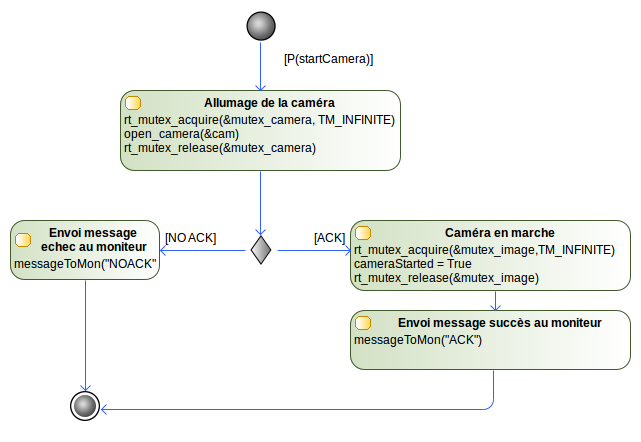
\includegraphics[width=0.8\textwidth]{./figures-pdf/th_startCamera}}
{\caption{Diagramme d'activité du thread {\tt th\_startCamera}}}
\end{center}
\end{figure}

\begin{figure}[H]
\label{fig:th_pictures}
\begin{center}
{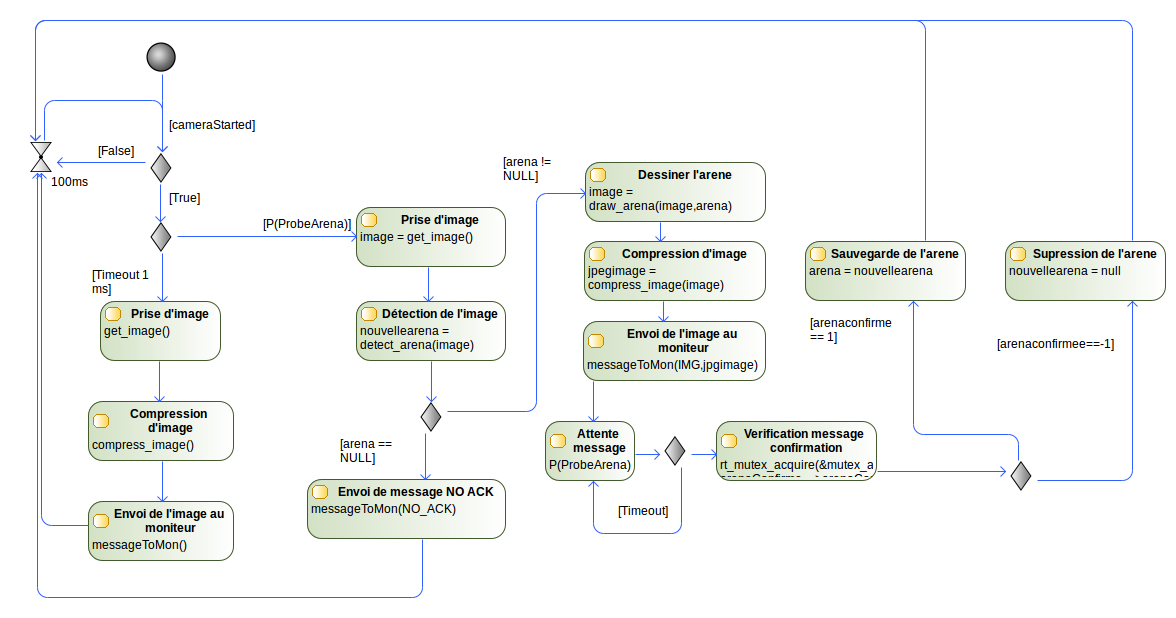
\includegraphics[width=1.0\textwidth]{./figures-pdf/th_pictures}}
{\caption{Diagramme d'activité du thread {\tt th\_pictures}}}
\end{center}
\end{figure}

% DIAGRAMME FONCTIONNEL GT ROBOT
\subsection{Groupe de threads gestion du robot}

% DIAGRAMME FONCTIONNEL GT ROBOT
\subsubsection{Diagramme fonctionnel du groupe gestion robot}

Voir \ref{fig:diag_fonc_gen_blocks}, {\color{blue} blocs de couleur bleue}.

% DESCRIPTION THREADS GT ROBOT
\subsubsection{Description des threads du groupe gestion robot}
%{\color{red} Remplissez le tableau ci-dessous pour expliquer le rôle de chaque thread et donner son niveau de priorité.}


\begin{table}[H]
\begin{center}
\begin{tabular}{|p{3cm}|p{8.5cm}|p{2cm}|}
\hline
\bf Nom du thread &	\bf Rôle &	\bf Priorité \\
\hline
\hline

th\_startRobot & Active et maintient le robot & 20\\
\hline
th\_batteryRobot & Rapporte l'état de la batterie du robot & 10\\
\hline
th\_openComRobot & Initialise la communication entre le robot et le moniteur & 20\\
\hline
th\_move & Transmet les commandes de mouvement du robot &	20\\
\hline
\end{tabular}
\end{center}
\caption{Description des threads du groupe {\tt th\_group\_gestion\_robot}}
\label{tab:gt_robot}
\end{table}

Les threads {\tt th\_move}, {\tt th\_batteryRobot} sont périodiques et ont un fonctionnement simple de transmission d'informations.\\

Le thread {\tt th\_openComRobot} ouvre le port série du module radio Xbee permettant la communication avec le robot.\\

Le thread {\tt th\_startRobot} a un fonctionnement un plus complexe puisqu'en outre du démarrage du robot selon le mode de fonctionnement demandé par le moniteur, il est hybride et s'occupe de la récupération sur incident en cas de pertes de trames de communication et des traitements associés au watchdog du robot.

% DIAGRAMMES D'ACTIVITE GT ROBOT
\subsubsection{Diagrammes d'activité du groupe robot}
%{\color{blue}Décrivez le comportement de chacun de vos threads avec des diagrammes d'activité. Apportez les explications qui vous semblent nécessaires pour comprendre votre conception.}

\begin{figure}[H]
\label{fig:th_startRobot}
\begin{center}
{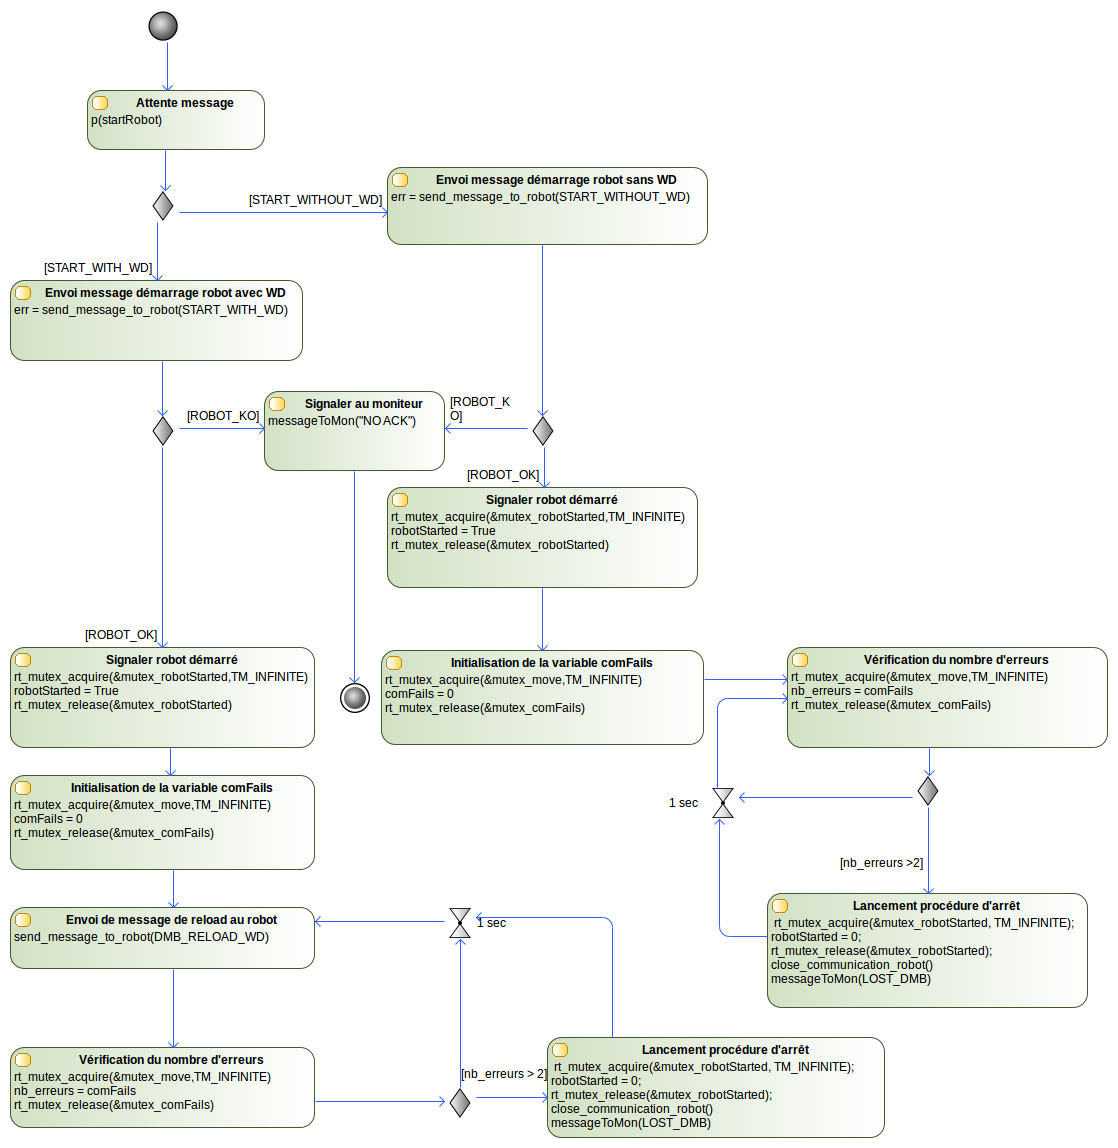
\includegraphics[width=1.0\textwidth]{./figures-pdf/th_startRobot}}
{\caption{Diagramme d'activité du thread {\tt th\_startRobot}}}
\end{center}
\end{figure}

\begin{figure}[H]
\label{fig:th_batteryRobot}
\begin{center}
{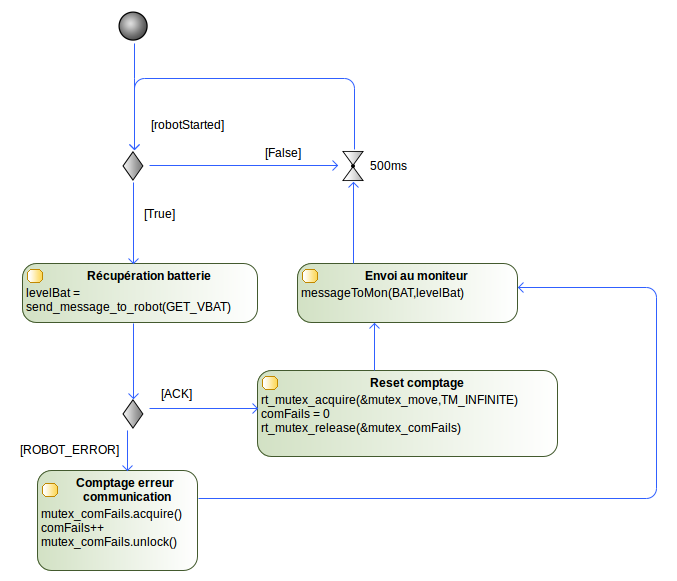
\includegraphics[width=1.0\textwidth]{./figures-pdf/th_batteryRobot}}
{\caption{Diagramme d'activité du thread {\tt th\_batteryRobot}}}
\end{center}
\end{figure}

\begin{figure}[H]
\label{fig:th_openComRobot}
\begin{center}
{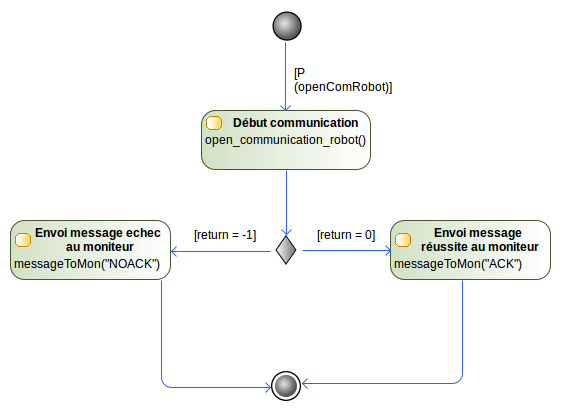
\includegraphics[width=0.8\textwidth]{./figures-pdf/th_openComRobot}}
{\caption{Diagramme d'activité du thread {\tt th\_openComRobot}}}
\end{center}
\end{figure}

\begin{figure}[H]
\label{fig:th_move}
\begin{center}
{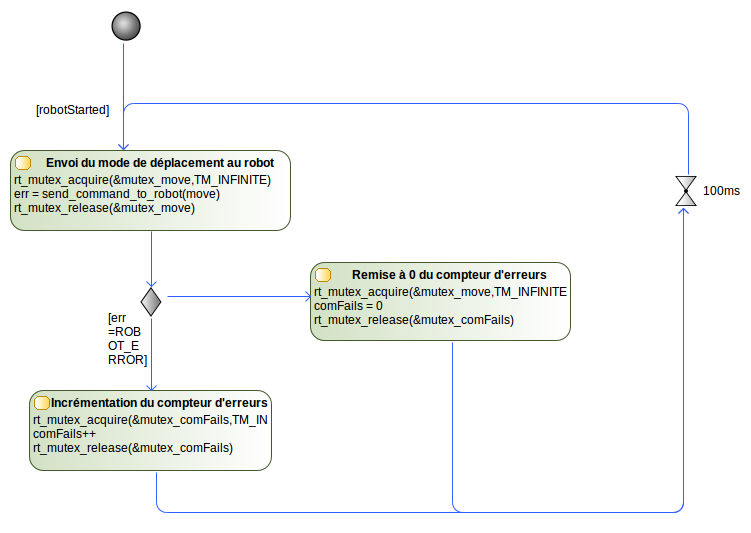
\includegraphics[width=0.85\textwidth]{./figures-pdf/th_move}}
{\caption{Diagramme d'activité du thread {\tt th\_move}}}
\end{center}
\end{figure}

%%%%%%%%%%%%%%%
% ANALYSE ET VALIDATION
\section{Analyse et validation de la conception}

\stepcounter{cptreq}
\subsection{Fonctionnalité \thecptreq}

\paragraph{Description :} Le lancement du serveur nodejs doit être réalisé au démarrage du superviseur. Le superviseur doit ensuite se mettre en attente de la connexion via le socket. En cas d'échec du démarrage du serveur nodejs, un message textuel doit être  affiché sur la console de lancement de l'application. Ce message doit signaler le problème et le superviseur doit s'arrêter.

\paragraph{\color{black}Réalisation :}  {\color{black} Fait en partie. La fonctionnalité est impléméntée sauf pour l'arrêt suite à l'échec de démarrage du serveur. L'implémentation actuelle stoppe la tâche en charge du démarrage du serveur, mais pas l'ensemble de l'application. Après discussion avec le client, la version actuelle est suffisante.}

\paragraph{\color{black}Remarques :}  {\color{black} Le démarrage du serveur NodeJS échoue trop souvent. L'origine de ce problème reste à diagnostiquer.}
%%%

\stepcounter{cptreq}
\subsection{Fonctionnalité \thecptreq}

\paragraph{Description :} La connexion entre nodejs et le superviseur (via le socket) doit être établie suite à la demande de connexion du moniteur.

\paragraph{\color{black}Réalisation :}  {\color{black} Réalisé \& validé.}

%%%

\stepcounter{cptreq}
\subsection{Fonctionnalité \thecptreq}

\paragraph{Description :} Tous les messages envoyés depuis le moniteur doivent être réceptionnés par le superviseur.

\paragraph{\color{black}Réalisation :} {\color{black} Réalisé \& validé.}
%%%
\stepcounter{cptreq}
\subsection{Fonctionnalité \thecptreq}

\paragraph{Description :} L'application superviseur doit être capable d'envoyer les messages au moniteur (via le serveur) avec un délai d'au plus 10~ms.

\paragraph{\color{black}Réalisation :} {\color{black} Réalisé.}

\paragraph{\color{black}Problèmes :} {\color{black} La fonction {\tt set\_msgToMon\_data} dont le rôle est de copier les données en charge utile du message transmis au moniteur est incorrecte. Elle alloue et copie des pointeurs vers la donnée à copier au lieu de cette dernière. Ce problème est critique et requiert correction. Il est possible de contourner ce problème en n'utilisant pas cette fonction.}

%%%
\stepcounter{cptreq}
\subsection{Fonctionnalité \thecptreq}

\paragraph{Description :} Le superviseur doit détecter la perte de communication avec NodeJS. En cas de perte de la communication un message doit être affiché sur la console de lancement du superviseur.

\paragraph{\color{black}Réalisation :} {\color{black} Réalisé \& validé. Traitement par le thread {\tt th\_cleaner}.}
%%%
\stepcounter{cptreq}
\subsection{Fonctionnalité \thecptreq}

\paragraph{Description :} En cas de perte de communication entre le superviseur et nodejs, il faut stopper le robot,  la communication avec le robot, le serveur nodejs et la camera afin de revenir dans le même état qu'au démarrage du superviseur.

\paragraph{\color{black}Réalisation :}  {\color{black} Réalisé \& validé. Traitement par le thread {\tt th\_cleaner} et par le processus principal du superviseur, qui est en attente permnanente d'une demande de réinitialisation intégrale des structures de données Xenomai et de leur redémarrage.}
%%%

\stepcounter{cptreq}
\subsection{Fonctionnalité \thecptreq}

\paragraph{Description :} Lorsque l'utilisateur demande, via le moniteur, à connecter le robot, la communication entre le superviseur et le robot doit être mise en place. Si la communication est active, il faut envoyer un message d'acquittement au moniteur. En cas d'échec, un message le signalant est renvoyé au moniteur.

\paragraph{\color{black}Réalisation :}  {\color{black} Réalisé \& validé.}

%%%
\stepcounter{cptreq}
\subsection{Fonctionnalité \thecptreq}

\paragraph{Description :} La communication entre le robot et le superviseur doit être surveillée par un mécanisme de compteur afin de détecter une perte du médium de communication.

\paragraph{\color{black}Réalisation :}  {\color{black} Réalisé \& validé. Les threads {\tt th\_battery} et {\tt th\_move} comptent toute trame non transmise au robot dans la variable partagée {\tt comFails}. Le thread {\tt th\_startRobot} vérifie périodiquement leur nombre et détecte à partir d'un certain seuil (3) une perte de communication.}

\paragraph{\color{black}Remarques :}  {\color{black} Le seuil de 3 trames perdues déclenchant l'état de perte de commucation est trop faible pour le médium utilisé. En effet Xbee utilise la bande des 2.4 GHz qui est très bruitée surtout dans un environnement de forte utilisation de technologies Wifi ou Bluetooth. La conséquence est que même à proximité directe de l'ordinateur de commande et du robot, ce seuil est rapidement atteint à cause du grand nombre de messages échangés par des threads à période courte.}
%%%
\stepcounter{cptreq}
\subsection{Fonctionnalité \thecptreq}

\paragraph{Description :} Lorsque la communication entre le robot et le superviseur est perdue, un message spécifique doit être envoyé au moniteur. Le système doit fermer la communication entre le robot et le superviseur et se remettre dans un état initial permettant de relancer la communication.

\paragraph{\color{black}Réalisation :}  {\color{black} Réalisé \& validé. Le thread {\tt th\_startRobot} ferme la communication avec le robot, arrête le traitement des tâches qui interagissent avec celui-ci et place le superviseur en état de relancer la connexion dès lors qu'une perte de communication avec le robot est déclarée.}

%%%

\stepcounter{cptreq}
\subsection{Fonctionnalité \thecptreq}

\paragraph{Description :} Lorsque l'utilisateur demande, via le moniteur, le démarrage sans watchdog, le robot doit démarrer dans ce mode. En cas de succès, un message d'acquittement est retourné à nodejs. En cas d'échec, un message indiquant l'échec est transmis à nodejs.

\paragraph{\color{black}Réalisation :}  {\color{black} Réalisé \& validé.}

%%%
\stepcounter{cptreq}
\subsection{Fonctionnalité \thecptreq}

\paragraph{Description :} Lorsque l'utilisateur demande, via le moniteur, le démarrage avec watchdog, le robot doit démarrer dans ce mode. Un message d'acquittement est retourné à nodejs. En cas d'échec, un message indiquant l'échec est transmis à nodejs.

Une fois le démarrage effectué, le robot doit rester vivant en envoyant régulièrement le message de rechargement du watchdog.

\paragraph{\color{black}Réalisation :}  {\color{black} Non réalisé. Le mécanisme de watchdog du robot ne fonctionne pas correctement et donc son implémentation par le superviseur est inutile.}

%%%
\stepcounter{cptreq}
\subsection{Fonctionnalité \thecptreq}

\paragraph{Description :} Lorsque qu'un ordre de mouvement est reçu par le superviseur, le robot doit réaliser ce déplacement en moins de 100~ms.

\paragraph{\color{black}Réalisation :} {\color{black} Réalisé \& validé. Cette fonctionnalité a été implémentée à l'aide d'une tâche qui envoie toutes les 100~ms un ordre de mouvement au robot une fois que celui-ci est démarré (tâche {\tt th\_move}). Cette implémentation ne garantit pas que le temps soit inférieur à 100~ms entre la réception du message et sa prise en compte par le robot. En effet, le temps de traitement de la réception par la tâche {\tt th\_receiveFromMon}, le temps de traitement de la tâche {\tt th\_move} et celui de l'envoi de l'ordre via le Xbee ne sont pas considérés. Afin de réduire ces délais, les priorités de  {\tt th\_receiveFromMon} et de {\tt th\_move} sont élevés mais ne permettent pas de garantir l'exigence de temps. Augmenter la fréquence de la tâche {\tt th\_move} permettrait de tenir cette contrainte, mais risque de surcharger la communication avec le robot (une version avec l'envoi de l'ordre que s'il a changé serait souhaitable). Finalement, une version asynchrone (attente d'un événement-donnée entre {\tt th\_receiveFromMon} et de {\tt th\_move}) aurait été préférable. Cependant, après discussion avec le client, la version périodique à 100~ms est cependant validée. }

%%%
\stepcounter{cptreq}
\subsection{Fonctionnalité \thecptreq}

\paragraph{Description :} Le niveau de la batterie du robot doit être mis à jour tous les 500~ms sur le moniteur.

\paragraph{\color{black}Réalisation :} {\color{black} Réalisé \& validé. Cette fonctionnalité a été implémentée à l'aide du thread périodique {\tt th\_battery} qui s'execute toutes les 500~ms.
Sa priorité est faible car ce n'est pas une tâche importante cependant la longue période et la nature très simple du traitement effectué garantit le respect de la contrainte temporelle. Ce thread ne s'exécute que si le robot est bien démarré, récupère l'état de sa batterie via la liaison sans fil puis la transmet au moniteur. }

\paragraph{\color{black}Remarques :} {\color{black} L'état de la batterie tel que reporté par le robot est un entier compris entre 0 et 2. Cette échelle de mesure est au mieux imprécise, au pire inadaptée. Une révision du firmware et/ou du circuit de mesure de la batterie du robot devrait être considérée.}

%%%
\stepcounter{cptreq}
\subsection{Fonctionnalité \thecptreq}

\paragraph{Description :} La camera doit être démarrée suite à une demande provenant du moniteur. Si l'ouverture de la  caméra a échoué, il faut envoyer un message au moniteur.

\paragraph{\color{black}Réalisation :} {\color{black} Réalisé \& validé.}

\paragraph{\color{black}Remarques :} {\color{black} Le démarrage de la caméra est un processus externe au superviseur qui prend 2 secondes à compléter. Dans certaines circonstances non définies ce processus peut échouer. Ce problème n'a cependant pas pu être reproduit et est considéré négligeable. Il est possible qu'il soit propre au matériel ou à l'implémentation du pilote de la caméra. }

%%%
\stepcounter{cptreq}
\subsection{Fonctionnalité \thecptreq}

\paragraph{Description :} Dès que la camera est ouverte, une image doit être envoyée au moniteur (via NodeJS) toutes les 100 ms.

\paragraph{\color{black}Réalisation :} {\color{black} Réalisé \& validé. Le thread {\tt th\_pictures} qui effectue ce traitement est périodique de période 100 ms. Malgré la nature lourde des traitements dont il a la charge, les tests n'ont pas permis de démontrer une incapacité à respecter cette contrainte temporelle.}

\paragraph{\color{black}Remarques :} {\color{black} Il est sans doute possible d'augmenter la période d'exécution de ce traitement pour obtenir un flux d'image plus rapide. Cependant l'utilisation d'un flux vidéo est plus adaptée que l'envoi d'images fixes; d'autant plus que l'ordinateur de supervision utilisée supporte l'encodage matériel AVC de flux haute définition.}

%%%
\stepcounter{cptreq}
\subsection{Fonctionnalité \thecptreq}

\paragraph{Description :} Suite à une demande de recherche de l'arène, le superviseur doit stopper l'envoi périodique des images, faire la recherche de l'arène et renvoyer une image sur laquelle est dessinée cette arène. Si aucune arène n'est trouvée un message d'échec est envoyé.\\

L'utilisateur doit ensuite valider visuellement via le moniteur si l'arène a bien été trouvée. L'utilisateur peut :
\begin{itemize}
	\item valider l'arène : dans ce cas, le superviseur doit sauvegarder l'arène trouvée (pour l'utiliser ultérieurement) puis retourner dans son mode d'envoi périodique des images en ajoutant à l'image l'arène dessinée.
 	\item annuler la recherche : dans ce cas, le superviseur doit simplement retourner dans son mode d'envoi périodique des images et invalider la recherche.
\end{itemize}

\paragraph{\color{black}Réalisation :} {\color{black} Réalisé \& validé. Le thread {\tt th\_pictures} qui est en charge du traitement des images est également en charge de cette fonctionnalité. Il interrompt la transmission des images capturées au moniteur en cas de déclenchement du processus de détection et de confirmation de l'arène.}

%%%
\stepcounter{cptreq}
\subsection{Fonctionnalité \thecptreq}

\paragraph{Description :} Suite à une demande de l'utilisateur de calculer la position du robot, le superviseur doit calculer cette position, dessiner sur l'image le résultat et envoyer un message au moniteur avec la position toutes les 100~ms. Si le robot n'a pas été trouvé, un message de position est envoyé avec une position (-1,-1).

\paragraph{\color{black}Réalisation :} {\color{black} Réalisé \& validé. Le thread {\tt th\_pictures} qui est en charge du traitement des images est également en charge de cette fonctionnalité. Comme ce traitement est effectuée par {\tt th\_pictures} lui-même de période 100 ms, le dessin de la localisation sur l'image capturée par la caméra et la transmission du message de position au moniteur est bien réalisé toutes les 100 ms.}
%%%
\stepcounter{cptreq}
\subsection{Fonctionnalité \thecptreq}

\paragraph{Description :} Suite à une demande de l'utilisateur de stopper le calcul de la position du robot, le superviseur doit rebasculer dans un mode d'envoi de l'image sans le calcul de la position.

\paragraph{\color{black}Réalisation :}  {\color{black} Réalisé \& validé. L'activation et la désactivation de la localisation du robot sont gérés par une variable partagée qui agit comme un interrupteur. Cette fonctionnalité n'a donc pas demandé plus de travail que la fonctionnalité précédente, ormis l'ajout du traitement du message de désactivation par le thread {\tt th\_receiveFromMon} de traitement des messages du moniteur.}

\end{document}